%!TEX TS-program = xelatex
%!TEX encoding = UTF-8 Unicode

%%
%% 使用 njuthesis 文档类生成南京大学本科生毕业论文的示例文档
%% 
%%

%% 
%% 南京大学本科学位论文模板
%% 2018年封面,摘要都发生了变化,本模板由以下2016年模板更改而来:http://haixing-hu.github.io/nju-thesis/

%% 如需Adobe字体请用(默认)
%\documentclass[adobefonts]{njuthesis}
%% MacOS系统请用
%\documentclass[macfonts]{njuthesis}
%% Windows系统请用
\documentclass[winfonts]{njuthesis}
%\usepackage{enumerate}
\usepackage{enumitem}
%% Linux系统请用
%\documentclass[linuxfonts]{njuthesis}
\newcommand\redbf[1]{\textbf{\textcolor{red}{#1}}}
\renewcommand{\today}{\number\year 年 \number\month 月 \number\day 日}
%%%%%%%%%%%%%%%%%%%%%%%%%%%%%%%%%%%%%%%%%%%%%%%%%%%%%%%%%%%%%%%%%%%%%%%%%%%%%%%
% 设置论文的中文封面
% 论文标题
\title{安卓不可见控件内存泄漏的自动检测}

% 论文作者姓名
\author{王冬杨}
% 论文作者学号
\studentid{161250136}
% 导师姓名职称
\supervisor{马骏}
% 导师职称
\supervisortitle{副教授}
% 论文作者院系
\department{软件学院}
% 论文作者专业方向
\major{软件工程}
% 论文作者的年级
\grade{2016级}
% 论文提交日期,需设置年、月、日。此属性可选,默认值为最后一次编译时的日期,精确到日。
\submitdate{\today}

%%%%%%%%%%%%%%%%%%%%%%%%%%%%%%%%%%%%%%%%%%%%%%%%%%%%%%%%%%%%%%%%%%%%%%%%%%%%%%%
% 设置论文的英文封面

% 论文的英文标题
\englishtitle{Thesis paper template}
% 论文作者姓名的拼音
\englishauthor{San Zhang}
% 导师姓名职称的英文
\englishsupervisor{Professor Si Li}
% 论文作者所在院系的英文名称
\englishdepartment{School of Electronic Science and Engineering}
% 论文作者所在学校或机构的英文名称。此属性可选,默认值为``Nanjing University''。
\englishinstitute{Nanjing University}
% 论文完成日期的英文形式,默认最后一次编译的时间
\englishdate{May 20, 2018}
% 专业
\englishinstitute{Electronic Information Science and Technology}
%%%%%%%%%%%%%%%%%%%%%%%%%%%%%%%%%%%%%%%%%%%%%%%%%%%%%%%%%%%%%%%%%%%%%%%%%%%%%%%
% 设置论文的页眉页脚
\usepackage{fancyhdr}
%\usepackage{enumitem}

\pagestyle{fancy}
%\lhead{\bfseries 141180092 }
\chead{安卓不可见控件内存泄漏的自动检测}
\rhead{王冬杨}
%\lfoot{From: K. Grant}
%\cfoot{To: Dean A. Smith}
%\rfoot{\thepage}
\renewcommand{\headrulewidth}{0.4pt}
%\renewcommand{\footrulewidth}{0.4pt}
%%%%%%%%%%%%%%%%%%%%%%%%%%%%%%%%%%%%%%%%%%%%%%%%%%%%%%%%%%%%%%%%%%%%%%%%%%%%%%%

\usepackage{xcolor}
\usepackage{minted}

\usepackage{listings}

\usepackage{color}
\definecolor{gray}{rgb}{0.4,0.4,0.4}
\definecolor{darkblue}{rgb}{0.0,0.0,0.6}
\definecolor{cyan}{rgb}{0.0,0.6,0.6}

\lstset{
	basicstyle=\ttfamily,
	columns=fullflexible,
	showstringspaces=false,
	commentstyle=\color{gray}\upshape
}
\begin{document}

% 制作中文封面
\maketitle
% 制作英文封面
% \makeenglishtitle
% 毕业论文过程管理四页表
% \controlpage %可以将word文件交给老师签字后扫描转成pdf,然后命名为controlpage.pdf

% 论文的中文摘要
\begin{abstract}

在安卓应用中,服务和广播得到了广泛应用,在绝大多数的商店应用当中,都可以找到服务和广播的应用,开发者可以使用这些组件方便地为应用提供诸如下载,数据更新,跨应用通信等不可缺少的重要功能。但是,服务和广播的广泛使用也具有一定的安全问题:由于服务和广播的开发具有碎片化以及不可见的特点,以及开发者经常忽视这些不可见控件的生命周期管理,因此在此类组件中发生内存泄漏的几率很高。而正由于这些组件的不可见的特性,使得内存泄漏问题的发现,解决的速度通常都比较慢,产生的影响的时间会比较长。

安卓官方也在逐渐重视这些不可见组件的生命周期管理:近期安卓系统在版本更新时,着重推出了“电池管理策略”,并在后续的版本更新中,对该策略进行了进一步的完善和升级。“电池管理策略”的主要目的是通过重点对后台不可见组件的行为进行了规范和约束,尽可能的节约电量消耗。这一策略会尽可能地促使开发者对不可见组件进行有效的生命周期控制,以减少内存泄漏发生的可能性,也会使开发者加大对不可见控件的测试力度,提前发现和解决更多的问题。但另一方面,这项更新会使得服务和广播的注册、启动方式都有了一定变化,这将会影响一些应用在新版本上的兼容性,同时也加重了碎片化现象。

在本文中,讨论并实现了一套针对安卓不可见控件的内存泄漏问题进行自动化检测诊断的工具,该工具可以在最新的安卓版本上进行检测,使用此自动检测工具可以帮助开发者快速方便的诊断应用中的服务和广播是否存在内存泄漏的问题,生成内存泄漏控件清单,以辅助开发者进行测试和调试。

同时本文在应用市场中下载了若干真实应用,使用本文开发的自动测试工具进行实验,发现在安卓应用中,组件的碎片化和内存泄漏问题较为普遍的存在。

在具体的实现上,该自动检测工具借助了开源工具\textbf{apktool}\cite{apktool}进行apk的反编译以得到应用的控件清单、\textbf{mat}\cite{mat}进行内存对象的分析以寻找内存泄漏的实例;使用安卓sdk中的\textbf{adb}和\textbf{emulator}等工具完成测试的流程;并使用\textbf{socket}来完成工作站与安卓模拟器的通信。

% 同时应该注意到,空白页是故意留白,以便章节开头能够出现在偶数页。
% 中文关键词。关键词之间用中文全角分号隔开,末尾无标点符号。
\keywords{安卓系统;内存泄漏;安卓服务;安卓广播}
\end{abstract}

%%%%%%%%%%%%%%%%%%%%%%%%%%%%%%%%%%%%%%%%%%%%%%%%%%%%%%%%%%%%%%%%%%%%%%%%%%%%%%%
% 论文的英文摘要
% \begin{englishabstract}
% The diversity of handwritten Chinese text make it a promising but % challenging computer vision problem. 
% 英文关键词。关键词之间用英文半角逗号隔开,末尾无符号。
% \englishkeywords{Handwritten Chinese, Text recognition, Deep learning}
% \end{englishabstract}

%%%%%%%%%%%%%%%%%%%%%%%%%%%%%%%%%%%%%%%%%%%%%%%%%%%%%%%%%%%%%%%%%%%%%%%%%%%%%%%
% 论文的前言,应放在目录之前,中英文摘要之后
%
%\begin{preface}
%
%在过去的40年中,手写中文文本领域识别(HCTR)取得了很大的进展[1,2]。
%
%\vspace{1cm}
%\begin{flushright}
%饶安逸\\
%2018年5月15日于南大仙林
%\end{flushright}
%
%\end{preface}

%%%%%%%%%%%%%%%%%%%%%%%%%%%%%%%%%%%%%%%%%%%%%%%%%%%%%%%%%%%%%%%%%%%%%%%%%%%%%%%
% 生成论文目录
\tableofcontents

%%%%%%%%%%%%%%%%%%%%%%%%%%%%%%%%%%%%%%%%%%%%%%%%%%%%%%%%%%%%%%%%%%%%%%%%%%%%%%%
% 生成插图清单。如无需插图清单则可注释掉下述语句。
%\listoffigures

%%%%%%%%%%%%%%%%%%%%%%%%%%%%%%%%%%%%%%%%%%%%%%%%%%%%%%%%%%%%%%%%%%%%%%%%%%%%%%%
% 生成附表清单。如无需附表清单则可注释掉下述语句。
%\listoftables

%%%%%%%%%%%%%%%%%%%%%%%%%%%%%%%%%%%%%%%%%%%%%%%%%%%%%%%%%%%%%%%%%%%%%%%%%%%%%%%
% 开始正文部分
\mainmatter

%%%%%%%%%%%%%%%%%%%%%%%%%%%%%%%%%%%%%%%%%%%%%%%%%%%%%%%%%%%%%%%%%%%%%%%%%%%%%%%
% 学位论文的正文应以《绪论》作为第一章
\chapter{绪论}\label{chapter_introduction}
\section{研究背景}
在安卓应用中,服务(Services)和广播(Broadcast)得到了广泛的使用。服务可以在安卓应用的后台保持长期运行,提供诸如下载、数据更新等重要功能。然而,正因为服务长期运行于后台的特点,使其往往容易产生异常(Errors)。如果服务的编写人员缺少警惕性,服务中出现的错误(Bug)可能会导致诸多问题,严重者可能引起应用崩溃,甚至系统死机;广播是一种常被用来进行跨应用的通信的通信手段,应用在使用广播进行与系统或者与其他应用进行通讯时,应用需要编写广播接收器(Broadcast Receiver)。负责运行广播接收器的时应用的主线程种,因此在广播接收器中不适合进行耗时操作,通常会在广播接收器中启动服务来进行后续的处理,因此广播接收器也可能通过服务或者自身导致内存泄漏。

安卓应用中的内存泄露指资源(内存对象、句柄、服务等)将不再被使用,但却无法被安卓系统的垃圾回收器(Garbage Collector)所回收,同时也是服务中的一大类常见问题。服务如果出现内存泄露,将会导致内存使用量意外大幅度增加,进而使得系统效率降低,严重影响用户体验。

有一类服务被称为\textbf{公开服务},即指定了\textbf{"exported:true"}属性的服务。其他应用在满足一定条件时(满足权限要求等)可以启动应用的公开服务,因此内存泄露的问题将会变得更加复杂。

由于在安卓8及更高的版本下,安卓操作系统的“电池优化策略”禁止跨应用启动后台服务\cite{android-service-limit},而这一方式在安卓7以及更早的版本中是可行的,因此在新版本(安卓8及更高)的安卓系统中,公开服务的内存泄漏检测方法与之前的方法\cite{jun2018lesdroid}有所差别,也正因为禁止跨应用启动后台服务,公开服务的内存泄漏问题也得到了很大的规避。

\section{相关工作}

Erika 等人在安卓8之前的版本中,编写了一个检测跨应用通信安全问题的工具Com Droid\cite{chin2011analyzing},文中阐述的方法对于跨应用测试具有指导意义。


在安卓8之前的版本中,跨应用启动服务这一行为是被允许的,南京大学的马骏等人安卓8之前的版本中,实现过一个公开服务(Exported Services)内存泄漏的检测工具LES Droid\cite{jun2018lesdroid},文中采用的方式分为四步:

\begin{enumerate}
	\item 使用apktool反编译工具\cite{apktool}对被测试应用进行反编译,获取被测试应用的安卓组件清单(AndroidManifest.xml)文件,解析获取应用中所有的公开服务的包名和类名。
	\item 将测试驱动应用、被测试应用通过adb安装到模拟器中,启动测试驱动应用。
	\item 测试驱动应用重复启动、关闭被测试的服务,在满足一定测试强度之后,导出被测试应用的堆镜像文件(.hprof files)。
	\item 基于MAT内存分析库\cite{mat}编写堆镜像文件的分析工具,自动检测内存泄漏并统计泄露的入口等。
\end{enumerate}

\label{pre-result}
文中的数据指出:在41537个被测试应用中,共在其中28662(69\%)个应用中检测出74831个服务,其中3934(13.7\%)个应用拥有公开服务。经过去重、安装测试以及应用商店评分筛选,有375个实际测试应用,最终通过不同的测试配置,最终检测到在18.7\%的应用中有16.8\%的服务存在内存泄漏问题。


\section{本文主要工作}
本文旨在探索一套适用于安卓8以上版本的公开服务和静态注册广播接收器的内存泄漏检测方法。主要工作如下:
\begin{enumerate}
\item 找到在安卓8以上版本的安卓系统上可行的跨应用测试方法。

\item 对桩应用上进行测试,并能发现所有泄露。

\item 在应用商店中下载真实应用,进行自动化测试分析实验结果。

\end{enumerate}
\section{本文结构}
本文的各章节组织结构如下:
\begin{itemize}
	\item[第一章] 绪论。简要说明了安卓组件内存泄漏的现象和后果。并概括地描述了检测安卓不可见控件内存泄漏的方法流程,总结了本文结构。
	\item[第二章] 背景
	\item[第三章] 自动化检测工具。
	\item[第四章] 实验。介绍了实验进行的配置环境,测试使用应用的来源,以及实验数据结果。
	\item[第五章] 总结与讨论。总结全文工作,讨论存在的问题和今后可以继续研究的方向。
\end{itemize}
\chapter{背景}\label{chapter_background}

本节将介绍本文的测试对象:安卓服务以及安卓广播接收器。
\section{安卓服务}

在安卓系统中,每个安卓应用都对应着一个主线程,这个主线程将负责处理界面计算和渲染、负责处理用户的交互以及负责响应生命周期事件等。这些任务对主线程产生了快速响应的要求,否则会导致用户体验质量的下降。换言之,在主线程中只能进行不耗时(几毫秒级别)的计算和操作,而任何耗时较长的计算和操作都必须在主线程之外的单独的后台线程之上来完成。这样可以使得用户在积极的与应用交互时,应用在后台可以积极的响应和运行。

然而,后台任务不可避免地将会使用安卓设备的资源:例如内存资源和电池电量等。如果后台任务操作不当(如占用大量内存导致系统卡顿,长期进行密集计算导致电池电量下降变快),也可能会导致用户体验下降;同时如果安卓服务的开发人员在开发时引入了\textbf{程序缺陷},使得服务在运行时产生了\textbf{内存泄漏},将会使得前面的现象变得更加严重。因此随着安卓系统的更新,其对服务组件也进行了更多的限制,以尽可能保证用户体验。

\begin{itemize}
	\item \textbf{安卓6.0(API 级别 23) } 引入了\textbf{低电量模式以及应用待机模式}。低电量模式会在屏幕关闭且设备处于静止状态时,对运行中应用的行为进行限制,以减少电量消耗,例如:限制网络访问,限制同步等。即当开启低电量模式时,服务的行为会受到一定程度的限制。
	\item \textbf{安卓7.0(API 级别 24)} 此版本限制了隐式广播的注册,并将上个版本中推出的低耗电模式推广成为一个随时进行的系统耗电优化:即当屏幕一段时间处于未唤醒状态且未接入电源,低耗电模式就会启动,而无需手动开启。即只要设备处于闲置状态时,服务的行为随时都会受到限制。
	\item \textbf{安卓8.0(API 级别 26)} 对后台服务的行为进行了更严格的限制,其中影响较大的一条规则是:\textbf{禁止处于后台的应用启动新的服务},取而代之的是需要显式经过用户许可,启动前台服务。这些限制对跨应用测试的研究带来了不便(跨应用测试一般由测试人员编写的测试驱动应用去启动其他(后台)应用的组件)。
	\textbf{安卓9.0(API 级别 28)} 引入了应用待机存储分区。系统将会根据应用的使用模式,来动态分配给应用使用资源的优先级。
\end{itemize}

本节接下来将会详细介绍服务的启动方式,生命周期,注册方式,以及内存泄漏的成因。

\subsection{服务的启动方式}
安卓应用中的服务可以通过两种方式启动\cite{service}:

\textbf{start 方式 } 其他组件构造特定的\textbf{Intent}对象,通过调用\textbf{startService() API}来启动目标服务。

\textbf{bind 方式 } 通过调用\textbf{bindService() API}将目标服务与特定组件绑定。被绑定的服务提供接口供其他组件与之交互。
一个服务可以同时通过以上两种方式启动。

\subsection{服务的生命周期}
服务的生命周期根据启动方式不同分为两种\cite{service}:

\textbf{start 方式 } 通过\textbf{startService() API}启动的服务将会一直运行,直到调用\textbf{stopSelf()}方法将自己停止运行。其他组件也可以通过调用\textbf{stopService() API}将服务停止运行。

停止运行的服务将会被\textbf{GC(Garbage Collector)}回收。

\textbf{bind 方式 } 通过\textbf{bindService() API}启动的服务将通过\textbf{IBinder}接口与其他组件进行交互,直到其他组件调用\textbf{unbindService() API}解除绑定。

一个服务可以同时绑定到多个组件之上,直到所有组件都解除了绑定时,该服务才会被\textbf{GC}回收。

每个安卓应用都关联一个\textbf{ActivityThread}实例,负责调度和执行该应用的各种组件。\textbf{ActivityThread}有一个\textbf{ArrayMap}类型的成员变量\textbf{mServices},其中保存了所有没有被销毁的服务的引用。一旦某个服务的实例被销毁,其引用将会从\textbf{mServices}中删除。

\subsection{服务的注册方式}
\begin{listing}[htbp]
	\centering
	\caption{服务的注册方式}
	\begin{minted}[encoding=utf8,
	frame=single,
	framesep = 1em,
	numbers=left, 
	breaklines=true, 
	tabsize=4,
	xleftmargin=2em,xrightmargin=2em,
	fontsize=\footnotesize]{xml}
<manifest
	xmlns:android="http://schemas.android.com/apk/res/android"
	xmlns:dist="http://schemas.android.com/apk/distribution"
	package="com.example.myapplication">
	<dist:module dist:instant="true" />
	<application ...>
		...
		<service android:name=".Service1"
			android:enabled="true"
			android:exported="true">
		</service>
		<service
			android:name = ".Service2"
			android:enabled = "true"
			android:exported = "false">
			<intent-filter>
				<category android:name = "cat1"/>
				<action android:name = "act2"/>
			</intent-filter>
		</service>
		<service android:name = ".Service3"
			android:enabled = "true"
			android:permission = "Permission1">
			<intent-filter>
				<action android:name = "act3"/>
				<category android:name = "cat2"/>
				<data android:scheme = "Scheme1"/>
				<data android:scheme = "Scheme2"/>
			</intent-filter>
		</service>
	</application>
</manifest>
	\end{minted}
	\label{declaration:service}
\end{listing}
通常,每个服务都要在\textbf{AndroidManifest.xml}中注册一个\textbf{<service>}标签(参考Listing.\textcolor{red}{\ref{declaration:service}}中的样例)。同时服务可以通过设置"\textbf{android:exported}"属性来指定该服务是否将被导出。当设置\textbf{android:exported = "true"}时,该服务可以被其他应用使用,反之不可。
%可以凑更多字数
\subsection{服务的内存泄漏}\label{service_leak}
通常,一个服务的实例不再被使用时应该被\textbf{GC(Garbage Collector)}回收,并释放资源。然而在某些情况下,一个被销毁的服务可能会意外的被引用,从而使得\textbf{GC}无法将其回收并释放资源,这样就造成了服务的内存泄漏。
\begin{listing}[htbp]
	\centering
	\caption{服务的内存泄漏}
	\begin{minted}[encoding=utf8,
	frame=single,
	framesep = 1em,
	numbers=left, 
	breaklines=true, 
	tabsize=4,
	showtabs = false,
	xleftmargin=2em,xrightmargin=2em,
	fontsize=\footnotesize]{java}
public class LeakedService extends Service{
	private static final String TAG = "LeakedService";
	// Method will be called when an instance is creating.
	public void onCreate(){
		...
		new Timer().scheduleAtFixedRate(new TimerTask(){
			public void run(){
				Log.d(TAG, LeakedService.this.getPackageName() + ".LeakedService is running!");
			}
		},1000L,3000L);
	}
	// Method will be called when an instance is destroying.
	public void onDestroy(){
		...
	}
}
	\end{minted}
	\label{leaked example:service}
\end{listing}

例如在游戏\emph{com.siendas.games2048}中,就出现了原理如图(见\textbf{Listing.\textcolor{red}{\ref{leaked example:service}}})的内存泄漏。具体导致内存泄露的原理为:在\textbf{LeakedService}的实例被构造的时候,将会调用他的\textbf{onCreate()}方法,在该方法中延迟\textbf{1000ms}启动了一个\textbf{匿名}计时器,该计时器将以\textbf{3000ms}的周期打印调试信息,可以看到在\textbf{TimerTask}类中持有了\textbf{LeakedService}的引用,而在该服务被销毁时,其\textbf{onDestroy()}方法中并没有对该匿名计时器进行销毁。因此在该服务被销毁后,将会一直存在一个匿名计时器持有该服务的引用,导致\textbf{GC}无法将其回收,从而导致了内存泄漏。

\section{安卓广播接收器}

安卓系统中,可以在安卓应用之间、以及安卓应用与安卓系统之间实现通讯,这种通讯的手段被称为广播\cite{androidbroadcastsguide},广播的设计采用了发布-订阅的设计模式。特定的广播将会在特定的事件发生时发送,例如:安卓系统将在各种系统事件(插拔耳机,插拔电源等)发生时发送系统广播;再如:一个安卓应用可以发送自定义的广播来同志其他的安卓应用,将一些消息传递给后者。

在使用广播时,应用需要注册接收特定的广播(称之为\textbf{订阅订阅})。在相应的广播发出,将由安卓系统负责将广播发送给订阅此种广播的应用。因此在安卓应用的角度,只需要订阅所需要的广播类型,以及关注在接收到广播时需要做出的响应动作即可,具有这种功能的组件被称为\textbf{广播接收器}。
	
一般而言,在跨应用通信时,广播是被广泛使用的一种方便的手段。但是在使用广播时需要格外小心,如果应用滥用广播,可能会导致系统运行变迟钝。更严重的,如果开发人员在编写广播接收器的时候引入\textbf{程序缺陷},将会导致更严重的问题(如应用崩溃等)。

本节接下来将会介绍广播接收器的启动方式,生命周期,注册方式,以及内存泄漏的成因。

\subsection{广播接收器的启动方式}
安卓应用中的广播接收器亦有两种方式启动\cite{broadcast}:

\textbf{清单声明的接收器 }\label{declaration:receiver in manifest} 通过在\textbf{AndroidManifest.xml}中添加\textbf{<receiver>}标签注册广播接收器,通过\textbf{<intent-filter>}标签指定接收器所订阅的广播操作。系统软件包管理器会在应用安装时注册接收器。然后,该接收器会成为应用的一个独立入口点,这意味着如果应用当前尚未运行,系统可以启动应用并发送广播。系统会创建新的\textbf{BroadcastReceiver}组件对象来处理它接收到的每个广播。次对象仅在调用\textbf{onReceive(Context, Intent)}期间有效。一旦从此方法返回代码,系统便会认为该组件不再活跃。

\textbf{上下文注册的接收器 }\label{declaration:receiver in context} 通过在代码中构造出\textbf{BroadReceiver}实例,以及\textbf{IntentFilter}实例来指定订阅的广播内容,调用\textbf{registerReceiver(BroadcastReceiver, IntentFilter) API}来注册接收器。只要上下文有效,通过改种方式注册的广播接收器就会接收广播。如果要停止接收广播,需要调用\textbf{unregisterReceiver(BroadcastReceiver) API}来注销广播接收器

\subsection{广播接收器的生命周期}

广播接收器的生命周期根据启动方式不同亦分为两种\cite{broadcast}:

\textbf{清单声明的接收器 } 静态注册的接收器生命周期不限于\textbf{Activity}甚至整个应用。即使应用并不在运行,接收器也可以接收到订阅的广播。将会在\textbf{onReceive()}方法结束后被销毁。


\textbf{上下文注册的接收器 } 上下文注册的接收器,其生命周期仅限于注册的上下文,例如在\textbf{Activity}上下文注册的接收器,在整个\textbf{Activity}存活期间可以持续接收广播;在应用上下文中注册的接收器,则会在整个应用运行期间都可以接收广播。需要注意的是:这种方式启动的接收器必须手动进行销毁,即调用\textbf{unregisterReceiver() API},否则在上下文失效时,系统会抛出异常(并不会导致应用崩溃),同时接收器会引发泄露(见图.\textcolor{red}{\ref{fig:broadcast_leak}})。

\begin{figure}[htbp]
	\centering
	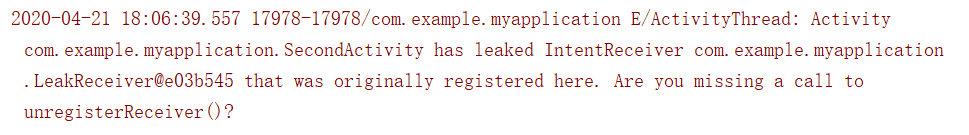
\includegraphics[width=0.9\textwidth]{broadcast_leak.png} % requires the graphicx package
	\caption{没有回收接收器将会导致异常以及泄露}
	\label{fig:broadcast_leak}
\end{figure}

\subsection{广播接收器的注册方式}
\begin{listing}[htbp]
	\centering
	\caption{广播接收器的注册方式}
	\begin{minted}[encoding=utf8,
	frame=single,
	framesep = 1em,
	numbers=left, 
	breaklines=true, 
	tabsize=4,
	showtabs = false,
	xleftmargin=2em,xrightmargin=2em,
	fontsize=\footnotesize]{XML}
<manifest 
	xmlns:android="http://schemas.android.com/apk/res/android"
	xmlns:dist="http://schemas.android.com/apk/distribution"
	package="com.example.myapplication">
	<dist:module dist:instant="true" />
	<application ...>
		...
		<receiver
			android:name = ".Receiver1">
			<intent-filter>
				<action android:name = "act1" />
			</intent-filter>
		</receiver>
		<receiver
			android:name = ".Receiver2"
			android:exported = "false"
			android:enabled = "true">
			<intent-filter>
				<category android:name = "cat1" />
				<action android:name = "act2" />
			</intent-filter>
		</receiver>
	</application>
</manifest>
	\end{minted}
	\label{declaration:receiver}
\end{listing}

一般而言,清单声明的广播接收器(见\ref{declaration:receiver in manifest})需要在\textbf{AndroidManifest.xml}文件中添加\textbf{<receiver>}标签(参考\textbf{Listing.\textcolor{red}{\ref{declaration:receiver}}}),在\textbf{<intent-filter>}子标签中可以指定订阅的广播内容等,也可以通过设置\textbf{"android:exported"}属性来指定该广播是否将被导出。而上下文注册的广播接收器(见\ref{declaration:receiver in context})则不需要进行前文的操作。
\subsection{广播接收器的内存泄漏}
广播接收器的内存泄漏原理类似与服务内存泄漏\ref{service_leak}。但是由广播接收器引起的内存泄漏往往比服务更为严重,因为广播接收器被系统认为只进行不耗时的操作(如果超过10s未从\textbf{onReceive()}方法中返回,将抛出\textbf{ANR Exception}),因此通常广播接收器在接到广播后,很有可能会启动其他的\textbf{Service}进行后续的耗时操作,进而可能会导致一连串的内存泄漏。

例如图中(见\textbf{Listing.\textcolor{red}{\ref{leaked example:receiver}}})所示的广播接收器,不仅本身会导致内存泄漏,而且还会启动一个会导致内存泄漏的服务(见\textbf{Listing.\textcolor{red}{\ref{leaked example:service}}}),因此后果将会更加严重。
\begin{listing}[htbp]
	\centering
	\caption{广播接收器的内存泄漏}
	\begin{minted}[encoding=utf8,
	frame=single,
	framesep = 1em,
	numbers=left, 
	breaklines=true, 
	tabsize=4,
	showtabs = false,
	xleftmargin=2em,xrightmargin=2em,
	fontsize=\footnotesize]{java}
public class LeakReceiver extends BroadcastReceiver {
	private final String TAG = "LeakReceiver";
	private final int ID = new Random().nextInt();
	@Override
	public void onReceive(Context context, Intent intent) {
		...
		context.startService(new Intent(context,LeakService.class));
		new Timer().scheduleAtFixedRate(new TimerTask() {
			@Override
			public void run() {
				Log.i(TAG,LeakReceiver.this.ID + " is running!");
			}
		}, 1000L, 3000L);
	}
}
	\end{minted}
	\label{leaked example:receiver}
\end{listing}

\chapter{自动化检测工具}\label{chapter_system}

本章将介绍安卓控件启动的流程,及检测内存泄露的原理。

\section{安卓服务}
安卓应用中的服务可以通过两种方式启动\cite{service}:

\textbf{start 方式 } 其他组件构造特定的\textbf{Intent}对象,通过调用\textbf{startService() API}来启动目标服务。

\textbf{bind 方式 } 通过调用\textbf{bindService() API}将目标服务与特定组件绑定。被绑定的服务提供接口供其他组件与之交互。
一个服务可以同时通过以上两种方式启动。

\subsection{服务的生命周期}
服务的生命周期根据启动方式不同分为两种\cite{service}:

\textbf{start 方式 } 通过\textbf{startService() API}启动的服务将会一直运行,直到调用\textbf{stopSelf()}方法将自己停止运行。其他组件也可以通过调用\textbf{stopService() API}将服务停止运行。

停止运行的服务将会被\textbf{GC(Garbage Collector)}回收。

\textbf{bind 方式 } 通过\textbf{bindService() API}启动的服务将通过\textbf{IBinder}接口与其他组件进行交互,直到其他组件调用\textbf{unbindService() API}解除绑定。

一个服务可以同时绑定到多个组件之上,直到所有组件都解除了绑定时,该服务才会被\textbf{GC}回收。

每个安卓应用都关联一个\textbf{ActivityThread}实例,负责调度和执行该应用的各种组件。\textbf{ActivityThread}有一个\textbf{ArrayMap}类型的成员变量\textbf{mServices},其中保存了所有没有被销毁的服务的引用。一旦某个服务的实例被销毁,其引用将会从\textbf{mServices}中删除。

\subsection{服务的注册方式}
\begin{listing}[htbp]
	\centering
	\caption{服务的注册方式}
	\begin{minted}[encoding=utf8,
	frame=single,
	framesep = 1em,
	numbers=left, 
	breaklines=true, 
	tabsize=4,
	xleftmargin=2em,xrightmargin=2em,
	fontsize=\footnotesize]{xml}
<manifest
    xmlns:android="http://schemas.android.com/apk/res/android"
    xmlns:dist="http://schemas.android.com/apk/distribution"
    package="com.example.myapplication">
    <dist:module dist:instant="true" />
    <application ...>
        ...
        <service android:name=".Service1"
            android:enabled="true"
            android:exported="true">
        </service>
        <service
            android:name = ".Service2"
            android:enabled = "true"
            android:exported = "false">
            <intent-filter>
                <category android:name = "cat1"/>
                <action android:name = "act2"/>
            </intent-filter>
        </service>
        <service android:name = ".Service3"
            android:enabled = "true"
            android:permission = "Permission1">
            <intent-filter>
                <action android:name = "act3"/>
                <category android:name = "cat2"/>
                <data android:scheme = "Scheme1"/>
                <data android:scheme = "Scheme2"/>
            </intent-filter>
        </service>
    </application>
</manifest>
	\end{minted}
	\label{declaration:service}
\end{listing}
通常,每个服务都要在\textbf{AndroidManifest.xml}中注册一个\textbf{<service>}标签(参考Listing.\textcolor{red}{\ref{declaration:service}}中的样例)。同时服务可以通过设置"\textbf{android:exported}"属性来指定该服务是否将被导出。当设置\textbf{android:exported = "true"}时,该服务可以被其他应用使用,反之不可。
%可以凑更多字数
\subsection{服务的内存泄漏}\label{service_leak}
通常,一个服务的实例不再被使用时应该被\textbf{GC(Garbage Collector)}回收,并释放资源。然而在某些情况下,一个被销毁的服务可能会意外的被引用,从而使得\textbf{GC}无法将其回收并释放资源,这样就造成了服务的内存泄漏。
\begin{listing}[htbp]
	\centering
	\caption{服务的内存泄漏}
	\begin{minted}[encoding=utf8,
		frame=single,
		framesep = 1em,
		numbers=left, 
		breaklines=true, 
		tabsize=4,
		showtabs = false,
		xleftmargin=2em,xrightmargin=2em,
		fontsize=\footnotesize]{java}
public class LeakedService extends Service{
	private static final String TAG = "LeakedService";
	// Method will be called when an instance is creating.
	public void onCreate(){
		...
		new Timer().scheduleAtFixedRate(new TimerTask(){
			public void run(){
				Log.d(TAG, LeakedService.this.getPackageName() + ".LeakedService is running!");
			}
		},1000L,3000L);
	}
	// Method will be called when an instance is destroying.
	public void onDestroy(){
		...
	}
}
	\end{minted}
	\label{leaked example:service}
\end{listing}

例如在游戏\emph{com.siendas.games2048}中,就出现了原理如图(见\textbf{Listing.\textcolor{red}{\ref{leaked example:service}}})的内存泄漏。具体导致内存泄露的原理为:在\textbf{LeakedService}的实例被构造的时候,将会调用他的\textbf{onCreate()}方法,在该方法中延迟\textbf{1000ms}启动了一个\textbf{匿名}计时器,该计时器将以\textbf{3000ms}的周期打印调试信息,可以看到在\textbf{TimerTask}类中持有了\textbf{LeakedService}的引用,而在该服务被销毁时,其\textbf{onDestroy()}方法中并没有对该匿名计时器进行销毁。因此在该服务被销毁后,将会一直存在一个匿名计时器持有该服务的引用,导致\textbf{GC}无法将其回收,从而导致了内存泄漏。

\section{安卓广播接收器}
安卓应用中的广播接收器亦有两种方式启动\cite{broadcast}:

\textbf{清单声明的接收器 }\label{declaration:receiver in manifest} 通过在\textbf{AndroidManifest.xml}中添加\textbf{<receiver>}标签注册广播接收器,通过\textbf{<intent-filter>}标签指定接收器所订阅的广播操作。系统软件包管理器会在应用安装时注册接收器。然后,该接收器会成为应用的一个独立入口点,这意味着如果应用当前尚未运行,系统可以启动应用并发送广播。系统会创建新的\textbf{BroadcastReceiver}组件对象来处理它接收到的每个广播。次对象仅在调用\textbf{onReceive(Context, Intent)}期间有效。一旦从此方法返回代码,系统便会认为该组件不再活跃。

\textbf{上下文注册的接收器 }\label{declaration:receiver in context} 通过在代码中构造出\textbf{BroadReceiver}实例,以及\textbf{IntentFilter}实例来指定订阅的广播内容,调用\textbf{registerReceiver(BroadcastReceiver, IntentFilter) API}来注册接收器。只要上下文有效,通过改种方式注册的广播接收器就会接收广播。如果要停止接收广播,需要调用\textbf{unregisterReceiver(BroadcastReceiver) API}来注销广播接收器

\subsection{广播接收器的生命周期}
广播接收器的生命周期根据启动方式不同亦分为两种\cite{broadcast}:

\textbf{清单声明的接收器 } 静态注册的接收器生命周期不限于\textbf{Activity}甚至整个应用。即使应用并不在运行,接收器也可以接收到订阅的广播。将会在\textbf{onReceive()}方法结束后被销毁。


\textbf{上下文注册的接收器 } 上下文注册的接收器,其生命周期仅限于注册的上下文,例如在\textbf{Activity}上下文注册的接收器,在整个\textbf{Activity}存活期间可以持续接收广播;在应用上下文中注册的接收器,则会在整个应用运行期间都可以接收广播。需要注意的是:这种方式启动的接收器必须手动进行销毁,即调用\textbf{unregisterReceiver() API},否则在上下文失效时,系统会抛出异常(并不会导致应用崩溃),同时接收器会引发泄露(见图.\textcolor{red}{\ref{fig:broadcast_leak}})。

\begin{figure}[htbp]
   \centering
   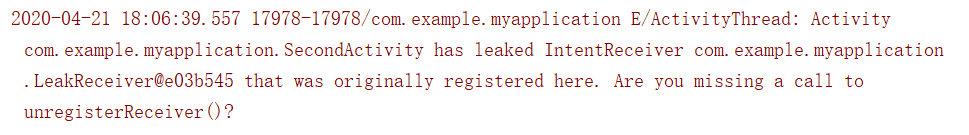
\includegraphics[width=0.9\textwidth]{broadcast_leak.png} % requires the graphicx package
   \caption{没有回收接收器将会导致异常以及泄露}
   \label{fig:broadcast_leak}
\end{figure}

\subsection{广播接收器的注册方式}
\begin{listing}[htbp]
	\centering
	\caption{广播接收器的注册方式}
	\begin{minted}[encoding=utf8,
	frame=single,
	framesep = 1em,
	numbers=left, 
	breaklines=true, 
	tabsize=4,
	showtabs = false,
	xleftmargin=2em,xrightmargin=2em,
	fontsize=\footnotesize]{XML}
<manifest 
	xmlns:android="http://schemas.android.com/apk/res/android"
	xmlns:dist="http://schemas.android.com/apk/distribution"
	package="com.example.myapplication">
	<dist:module dist:instant="true" />
	<application ...>
		...
		<receiver
			android:name = ".Receiver1">
			<intent-filter>
				<action android:name = "act1" />
			</intent-filter>
		</receiver>
		<receiver
			android:name = ".Receiver2"
			android:exported = "false"
			android:enabled = "true">
			<intent-filter>
				<category android:name = "cat1" />
				<action android:name = "act2" />
			</intent-filter>
		</receiver>
	</application>
</manifest>
	\end{minted}
	\label{declaration:receiver}
\end{listing}

一般而言,清单声明的广播接收器(见\ref{declaration:receiver in manifest})需要在\textbf{AndroidManifest.xml}文件中添加\textbf{<receiver>}标签(参考\textbf{Listing.\textcolor{red}{\ref{declaration:receiver}}}),在\textbf{<intent-filter>}子标签中可以指定订阅的广播内容等,也可以通过设置\textbf{"android:exported"}属性来指定该广播是否将被导出。而上下文注册的广播接收器(见\ref{declaration:receiver in context})则不需要进行前文的操作。
\subsection{广播接收器的内存泄漏}
广播接收器的内存泄漏原理类似与服务内存泄漏\ref{service_leak}。但是由广播接收器引起的内存泄漏往往比服务更为严重,因为广播接收器被系统认为只进行不耗时的操作(如果超过10s未从\textbf{onReceive()}方法中返回,将抛出\textbf{ANR Exception}),因此通常广播接收器在接到广播后,很有可能会启动其他的\textbf{Service}进行后续的耗时操作,进而可能会导致一连串的内存泄漏。

例如图中(见\textbf{Listing.\textcolor{red}{\ref{leaked example:receiver}}})所示的广播接收器,不仅本身会导致内存泄漏,而且还会启动一个会导致内存泄漏的服务(见\textbf{Listing.\textcolor{red}{\ref{leaked example:service}}}),因此后果将会更加严重。
\begin{listing}[htbp]
	\centering
	\caption{广播接收器的内存泄漏}
	\begin{minted}[encoding=utf8,
	frame=single,
	framesep = 1em,
	numbers=left, 
	breaklines=true, 
	tabsize=4,
	showtabs = false,
	xleftmargin=2em,xrightmargin=2em,
	fontsize=\footnotesize]{java}
public class LeakReceiver extends BroadcastReceiver {
	private final String TAG = "LeakReceiver";
	private final int ID = new Random().nextInt();
	@Override
	public void onReceive(Context context, Intent intent) {
		...
		context.startService(new Intent(context,LeakService.class));
		new Timer().scheduleAtFixedRate(new TimerTask() {
			@Override
			public void run() {
				Log.i(TAG,LeakReceiver.this.ID + " is running!");
			}
		}, 1000L, 3000L);
	}
}
	\end{minted}
	\label{leaked example:receiver}
\end{listing}
\section{自动化检测工具原理}


\chapter{实验}\label{chapter_experiment}
为了验证自动化检测工具的可行性、正确性,在本章中将设计实验进行验证。

首先将会设计仿真测试,在仿真测试中,会设计轻量级的、最简单的仿真应用,以检验自动检测工具是否能够正确检测出内存泄漏的组件,同时不出现误检的行为。

接下来为了评价在安卓10上服务和广播接收器的内存泄漏情况,将会从安卓应用市场中下载真实的应用,使用本文所述的工具进行测试,得出结论。
\section{仿真测试}

\subsection{仿真应用}

仿真应用(见\textbf{Listing.}\redbf{\ref{code: manifest}})应同时具有两个\textbf{公开服务}以及两个\textbf{清单声明的广播接收器}。其中每个控件之一需要人为制造内存泄漏(称为\textbf{LeakedService(Listing.\redbf{\ref{code:LeakedService}})}与\textbf{LeakedReceiver(Listing.\redbf{\ref{code:LeakedReceiver}})}),另一个则需要确保不存在内存泄漏(称为\textbf{NormalService(Listing.\redbf{\ref{code:Normal}})}与\textbf{NormalReceiver(Listing.\redbf{\ref{code:Normal}})})。
在对仿真应用进行测试时,预期的实验结果为:能够检测到\textbf{LeakedService}和\textbf{LeakedReceiver}的泄露实例,以证明该工具可以发现内存泄漏问题;而检测不到\textbf{NormalService}和\textbf{NormalReceiver}的泄露实例,以证明该工具不会将正常的组件误检。


\begin{listing}[htbp]
	\centering
	\caption{\textbf{LeakedService}主体代码}
	\begin{minted}[encoding=utf8,
	frame=single,
	framesep = 1em,
	numbers=left, 
	breaklines=true, 
	tabsize=4,
	xleftmargin=2em,xrightmargin=2em,
	fontsize=\footnotesize]{java}
public class LeakedService extends Service {
	private static final String TAG = "LeakedService";
	@Override
	public void onCreate() {
		super.onCreate();
		new Timer().scheduleAtFixedRate(new TimerTask() {
			@Override
			public void run() {
				Log.i(TAG,LeakService.this.getPackageName() + ".LeakService running ");
			}
		},1000L,3000L);
	}
}	
	\end{minted}
	\label{code:LeakedService}
\end{listing}

\begin{listing}[htbp]
	\centering
	\caption{\textbf{LeakedReceiver}主体代码}
	\begin{minted}[encoding=utf8,
	frame=single,
	framesep = 1em,
	numbers=left, 
	breaklines=true, 
	tabsize=4,
	xleftmargin=2em,xrightmargin=2em,
	fontsize=\footnotesize]{java}
public class LeakedReceiver extends BroadcastReceiver {
	private static final String TAG = "LeakedReceiver";
	private final Random random = new Random();
	@Override
	public void onReceive(Context context, Intent intent) {
		new Timer().scheduleAtFixedRate(new TimerTask() {
			@Override
			public void run() {
				Log.i(TAG,LeakReceiver.this.random.nextInt() + ".LeakReceiver running ");
			}
		},1000L,3000L);
	}
}
	\end{minted}
	\label{code:LeakedReceiver}
\end{listing}

\begin{listing}[htbp]
	\centering
	\caption{\textbf{NormalReceiver}与\textbf{NormalService}主体代码}
	\begin{minted}[encoding=utf8,
	frame=single,
	framesep = 1em,
	numbers=left, 
	breaklines=true, 
	tabsize=4,
	xleftmargin=2em,xrightmargin=2em,
	fontsize=\footnotesize]{java}
public class NormalReceiver extends BroadcastReceiver {
	private static final String TAG = "NormalReceiver";
	private final Random random = new Random();
	@Override
	public void onReceive(Context context, Intent intent) {
		Log.i(TAG,NormalReceiver.this.random.nextInt() + ".NormalReceiver running ");
		}
	}
}

public class NormalService extends Service{
	private static final String TAG = "NormalService";
		@Override
	public void onReceive(Context context, Intent intent) {
		Log.i(TAG,NormalService.this.getPackageName() + ".LeakService running ");
	}
}
	\end{minted}
	\label{code:Normal}
\end{listing}

\begin{listing}[htbp]
	\centering
	\caption{仿真应用的AndroidManifest.xml清单}
	\begin{minted}[encoding=utf8,
	frame=single,
	framesep = 1em,
	numbers=left, 
	breaklines=true, 
	tabsize=4,
	xleftmargin=2em,xrightmargin=2em,
	fontsize=\footnotesize]{xml}
<manifest
	xmlns:android="http://schemas.android.com/apk/res/android"
	xmlns:dist="http://schemas.android.com/apk/distribution"
	package="com.example.myapplication">
	<dist:module dist:instant="true" />

	<permission
		android:name="app.custom.permission"
		android:protectionLevel="signature" />
	<application ...>
		<activity android:name=".MainActivity">
			<intent-filter>
				<action android:name="android.intent.action.MAIN" />
				<category android:name="android.intent.category.LAUNCHER" />
			</intent-filter>
		</activity>
		
		<receiver
			android:name=".LeakedReceiver"
			android:exported="true">
			<intent-filter>
				<action android:name="TestActionForLeaked" />
			</intent-filter>
		</receiver>
		
		<receiver
			android:name = ".NormalReceiver"
			android:exported = "true">
			<intent-filter>
				<action android:name = "TestActionForNormal"/>
			</intent-filter>
		</receiver>
		
		<service
			android:name=".LeakedService"
			android:exported="true">
		</service>
	
		<service
			android:name = ".NormalService"
			android:exported = "true">
		</service>
	</application>
</manifest>
	\end{minted}
	\label{code: manifest}
\end{listing}

\subsection{实验结果}
实验结果(见\textbf{图.}\redbf{\ref{fig:result of mock receiver}}及\textbf{图.}\redbf{\ref{fig:result of mock service}})能正确检测到\textbf{LeakedService}和\textbf{LeakedReceiver}的内存泄漏实例,而没有误检\textbf{NormalService}以及\textbf{NormalReceiver},证明检测工具实际有效。

\begin{figure}[htbp]
	\centering
	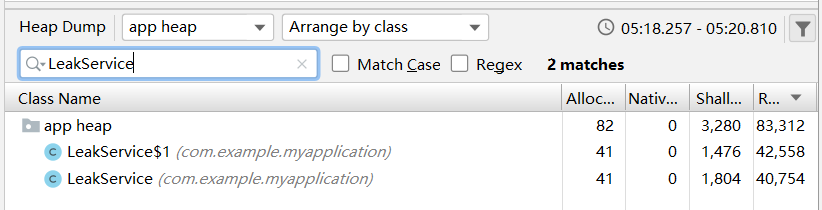
\includegraphics[width=0.9\textwidth]{service_leak_result.png} % requires the graphicx package
	\caption{检测到\textbf{LeakedService}内存泄漏实例}
	\label{fig:result of mock service}
\end{figure}
\begin{figure}[htbp]
\centering
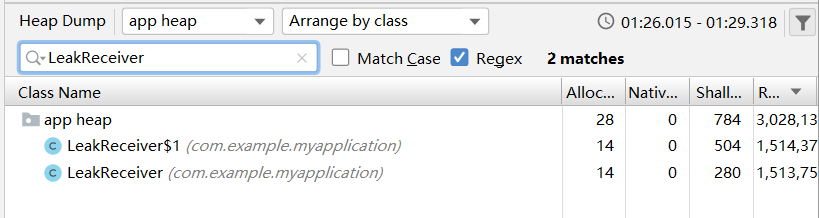
\includegraphics[width=0.9\textwidth]{receiver_leak_result.png} % requires the graphicx package
\caption{检测到\textbf{LeakedReceiver}内存泄漏实例}
\label{fig:result of mock receiver}
\end{figure}

\newpage
\section{真实测试}


本文选取了\textbf{AppChina 应用市场}\cite{appchina}作为测试应用的来源,在其中的\textbf{视频},\textbf{游戏},\textbf{工具}三个类别中,选取了每个分类中当月下载量最高的若干应用进行测试,共计\textbf{22}个。对这\textbf{22}个应用的测试结果详见\textbf{\redbf{\ref{now-result}}小节}:

\subsection{实验结果}\label{now-result}
\textbf{表现正常 12(54.5\%) }这些应用的组件表现正常,并没有出现内存泄露问题。

\textbf{内存泄漏 3(13.6\%) }这些应用包含了存在内存泄漏问题的组件,并成功被检测工具检测到。

\textbf{应用崩溃 7(31.8\%) }这些应用在测试时抛出了\textbf{ANR(Application Not Response)}异常,导致应用崩溃,无法完成测试。

\subsection{应用崩溃主要原因分析}

\textbf{无法正常启动 } 部分应用在启动时即发生了崩溃,导致应用停止运行。这类应用崩溃的原因可能是应用的版本和模拟器系统的版本不兼容,例如使用了不再符合开发规范的接口,某些接口不再支持,或没有在\textbf{AndroidManifest.xml}中声明所需的权限(缺少\textbf{<uses-permission>}标签)等。

\textbf{在测试过程中崩溃 } 部分应用可以正常启动,但是在\textbf{主测试流程}中发生了应用崩溃问题。这类应用崩溃的原因可能是因为应用的组件启动流程存在问题,比如:进行了风险操作,进行了线程不安全操作,没有对启动环境进行检查等;也可能是由于应用的组件确实存在\textbf{内存泄漏}问题,而且泄露表现的十分严重,触发了安卓系统的安全限制,导致安卓系统介入将应用停止运行。

\textbf{空指针异常 } 部分应用的组件在启动时会抛出\textbf{NullPointerException},该异常表示,在组件的启动过程中,对未实例化的对象进行了读写操作。这类问题大多数是因为组件的开发人员的疏忽,导致的程序缺陷。可能的成因有组件之间使用了共享资源,但是并没有进行专门管理,也有可能是因为这类组件的启动严格遵循\textbf{状态自动机},但是测试时无法得知组件启动需要满足的前置条件,导致运行出错。

\section{结果分析}

本小节会将本文的测试结果(见\ref{now-result})计算指标来进行分析。

\subsection{数据分析}
\begin{table}[htb]\footnotesize
	\centering
	\caption{实验数据及指标}
	\vspace{2mm}
	% l - left, r - right, c - center. | means one vertical line 这里声明的是表格单元中的内容如何对齐
	\begin{tabular}{lcccc}
		\toprule
		&\textbf{表现正常}&\textbf{内存泄漏}&\textbf{运行异常}&\textbf{泄露正常比}\\
		\midrule
		\textbf{指标}&54.5\%&13.6\%&31.8\%&0.250\\
		\bottomrule
	\end{tabular}
	\label{table:compare}
\end{table}

实验数据的对比表明:
\begin{itemize}
	\item 存在内存泄漏的应用比例为\textbf{13.6\%},说明组件内存泄漏现象较为普遍。
	\item 运行异常的应用比例为\textbf{31.8\%},说明安卓组件碎片化问题比较严重,兼容性问题相对于内存泄漏问题更为明显。兼容性问题具体原因有:安卓版本升级后,系统权限的收紧,导致应用无法像先前版本一样正常获取响应权限;组件的开发规范变更,导致原有代码抛出异常,导致应用崩溃等。
	\item 泄露正常比(检测到内存泄漏问题的应用数量与表现正常的应用数量之比)为\textbf{0.250},这项指标相较于\textbf{内存泄漏应用的比例}更有实际意义,它说明了在\textbf{经过成熟测试的稳定可用的应用}中,组件的内存泄漏问题依然较为普遍,这要求开发者在进行不可见组件开发的时候,需要投入更多的精力进行测试和调试,以确保这些组件中不会出现程序缺陷。
\end{itemize}

\subsection{实验数据局限性}

由于实验设备和实验环境的限制(参考\textbf{表.}\redbf{\ref{table:pc-compare}}),本文只能使用效率较慢的方式对少量小规模的应用进行串行的测试(参考\textbf{表.}\redbf{\ref{table:method-compare}})。因此实验结果具有较大的局限性。
\newline

\begin{table}[htb]\footnotesize
	\centering
	\caption{工作站配置}
	\vspace{2mm}
	% l - left, r - right, c - center. | means one vertical line 这里声明的是表格单元中的内容如何对齐
	\begin{tabular}{lcccc}
		\toprule
		&\textbf{操作系统}&\textbf{内存容量}&\textbf{处理器型号}&\textbf{模拟器系统版本}\\
		\midrule
		\textbf{测试配置}&Windows 10&8 GB&Intel(R) Core(TM) i7-8565U&Android 10\\
		\bottomrule
	\end{tabular}
	\label{table:pc-compare}
\end{table}

\begin{table}[htb]\footnotesize
	\centering
	\caption{测试方法}
	\vspace{2mm}
	% l - left, r - right, c - center. | means one vertical line 这里声明的是表格单元中的内容如何对齐
	\begin{tabular}{lcccc}
		\toprule
		&\textbf{并发能力}&\textbf{模拟器内存}&\textbf{模拟器SD卡容量}&\textbf{测试强度}\\
		\midrule
		\textbf{测试方法}&单线程&2 GB&512 MB&每个应用测试2次\\
		\bottomrule
	\end{tabular}
	\label{table:method-compare}
\end{table}

\section{小结}
在本章中,设计了仿真测试实验,以及真实测试实验。前者验证了自动化检测工具的正确性和可行性,而后者研究了安卓10中,应用的组件内存泄漏的发生几率,一定程度上验证了安卓组件开发碎片化的问题,同时证明安卓不可见控件内存泄漏的问题依然广泛存在。
\chapter{结论}\label{chapter_conclusion}
本文实现了一个自动化的检测工具,它可以帮助安卓应用的开发人员对应用进行测试,帮助发现存在内存泄露问题的公开服务以及清单声明的广播接收器,尽量减少应用中的缺陷和错误。

在本文的解决方案中,首先对被测试应用进行反编译,接下来编写了脚本分析应用组件清单,得到公开服务和清单声明的广播接收器的列表,作为被测试对象。之后启动安卓模拟器,将被测试应用、测试驱动应用安装到模拟器上,并启动测试驱动应用来负责执行整个测试任务:对被测试组件进行反复的启动/关闭,绑定/解绑定,注册/解注册操作,最大程度确保内存泄漏问题被实际触发。最后寻找内存泄漏的组件,将被测试应用的堆镜像文件导出到工作站中,基于开源工具开发了检测安卓组件内存泄漏的定制工具,最终导出组件的内存泄漏情况报告,以指导开发者对应用进行进一步的测试和调试工作。

但是本文的工作也存在相应的不足:如在实验的测试环节,由于工作站配置的制约,选取的应用数量和规模都很小,因此测试数据具有较大的偶然性;由于难度较大,本文针对广播接收器的测试中,只选取了在清单中注册的广播接收器进行测试,而没有对动态注册的广播接收器进行测试。

在未来的工作中,针对本文的上述不足大致有两个改进的方向:第一,针对测试不充分的问题,可以将本文的测试方法进行并行化的改进,然后使用更大量的应用进行充分的测试,来统计实验数据,这样会更有说服力。第二,对于动态注册的广播接收器,由于无法在清单中自动分析出这些接收器,且注册的过程相对比较复杂,可以寻找一些新的方式去对这一部分接收器进行测试;同理,内容提供器也属于安卓应用的不可见控件,而且也很容易出现内存泄漏的问题,因此对于内容提供器内存泄漏的检测也是未来工作的方向之一。

\bibliography{sample}

%%%%%%%%%%%%%%%%%%%%%%%%%%%%%%%%%%%%%%%%%%%%%%%%%%%%%%%%%%%%%%%%%%%%%%%%%%%%%%%
% 致谢,应放在结论之后
\begin{acknowledgement}
由衷地感谢我的导师马骏副教授对我进行了悉心的指导,恩施思维敏捷,脚踏实地,对我实验过程中遇到的苦难和疑惑,都进行了仔细耐心的讲解和指导,对我的毕业设计的完成给与了巨大的帮助。

我也要感谢实验室的同学们,在三年的训练中,我们一起互相帮助,同甘共苦,攻坚克难,是我奋斗路上可靠的队友。愿我们的友谊地久天长,愿你们今后取得更高的成就。

另外,我还要感谢开源社区中无数勤劳无私的贡献者们,没有你们开发的众多的开源工具,本文的工作无法完成。在此感谢开源工作者,以及众多博主的技术博客,让我学到了很多。

最后,还要感谢我的家人,无论我身在哪里,家人都一如既往的支持鼓励着我,是我前进路上最坚强的后盾。

感谢所有支持帮助我的人,也祝各位同学前途无量。
\end{acknowledgement}

%%%%%%%%%%%%%%%%%%%%%%%%%%%%%%%%%%%%%%%%%%%%%%%%%%%%%%%%%%%%%%%%%%%%%%%%%%%%%%%
\end{document}
